\documentclass{exam}

\usepackage{graphicx}
\usepackage[fleqn]{amsmath}
\usepackage{cancel}
\usepackage{polynom}
\usepackage{float}
\usepackage{mdwlist}
\usepackage{booktabs}
\usepackage{cancel}
\usepackage{polynom}
\usepackage{caption}

\newcommand{\degree}{\ensuremath{^\circ}} 

% \begin{figure}[H]
%   \centering
%   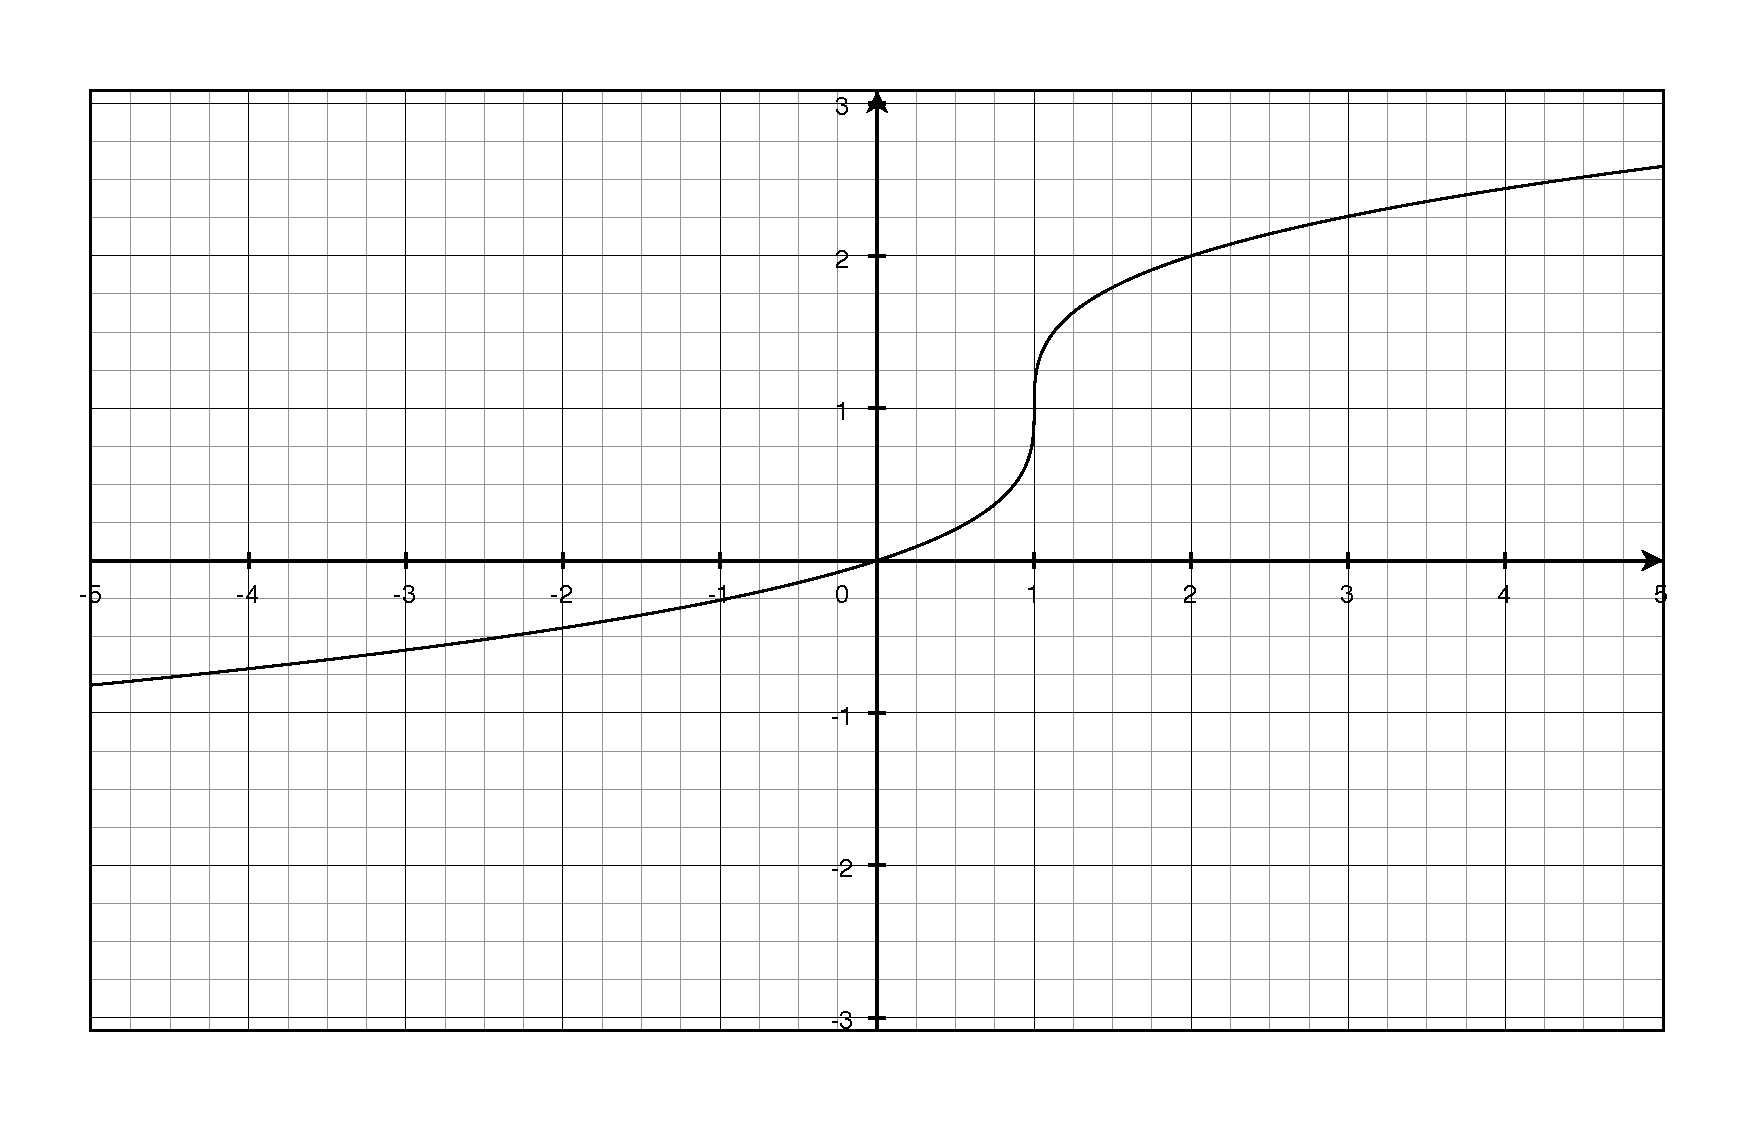
\includegraphics[scale=.3]{question7.eps}
%   \caption*{Question 7}
% \end{figure}

% \oddsidemargin .5in
% \topmargin -1in
\textwidth 6.5 in

\printanswers

\ifprintanswers 
\usepackage{2in1, lscape} 
\fi

\title{Physics \\ Homework One}
\date{September 12, 2011}
% \author{Ed Tellman}

\begin{document}

\maketitle

\ifprintanswers
\else
\section{Calculators}

Some of the problems require a calculator.  If you don't have one, you can borrow of the UBB
calculators at the PAB.  Let me know if access to calculators is difficult.

\fi

\section{From the Book}

\begin{itemize*}
  \item Read Chapters 2 and 3 of {\em The Physics of Everyday Phenomena}.
  \item pp 34-37: questions 8, 11, 14, 18, 19, 26; exercises 10, 15, 18; synthesis problem 2
  \item pp 53-55: questions 9-11, 13, 14, 20, 23; exercises 1, 2, 7, 8, and 14, synthesis problems 1 and 3
\end{itemize*}

\ifprintanswers
\section{Solutions}

\subsection{Chapter 2}

\begin{description}

\item[Q8]
The radar gun measures instantaneous speed and the plane measures average speed.

A driver observed by the plane could actually exceed the speed limit and not get a ticket.  He would just have to make
sure that he also spent some time stopped or driving slowly, so that his average speed was still OK.

Assuming all the equipment is accurate, neither method will result in someone unfairly getting a ticket.  The speed
limit is for instantaneous speed and the average speed is always somewhere between the highest and lowest instantaneous
speeds.

\item[Q11]
\begin{description*}
  \item[a] the velocity is not constant because both the speed and the direction are changing
  \item[b] the speed increases at the bottom of the swing and decreases at the ends when the ball changes direction
\end{description*}

\item[Q14]
Either car might or might not be accelerating---there is not enough information to tell.

\item[Q18]
\begin{description*}
  \item[a] The velocity is constant for the first 2 seconds.
  \item[b] The velocity is changing most rapidly between seconds 2 and 4.  This is the part of the graph with the
    steepest slope
\end{description*}

\item[Q19]
\begin{description*}
  \item[a] The distance is decreasing towards the end of the time, so the car is going backwards during this interval. 
  \item[b] The slope at point A is steeper than the slope at point B, so the velocity is greater at point A.
\end{description*}

\item[Q26]
If the acceleration was constant the velocity graph would be a straight line.  Since the velocity graph is curved, the
acceleration is not constant.

%% \item[E1]
%% \[
%%   S_{avg} = \frac{460 \text{ miles}}{8 \text{ hours}} = 57.5 \text{ mph}
%% \]

\item[E10]
\[
  a = \frac{7 \text{ m/s}}{2 \text{ s}} = 3.5 \text{ m/s}^2
\]

\item[E15]
\begin{description*}
\item[a] 
\begin{align*}
  v &= v_0 + at \\
   &= 30 \text{ m/s} - (3 \text{ m/s}^2) (3 \text{ s}) \\ 
   &= 21 \text{ m/s} \\
\end{align*}

\item[b] 
\begin{align*}
  d &= v_0t + \frac{1}{2} at^2 \\
   &= (30 \text{ m/s})(3 \text{ s}) + \frac{1}{2} (-3 \text{ m/s}^2)(3 \text{ s})^2 \\
   &= 76.5 \text{ m} \\
\end{align*}

\end{description*}

\item[E18]
\begin{figure}[H]
  \centering
  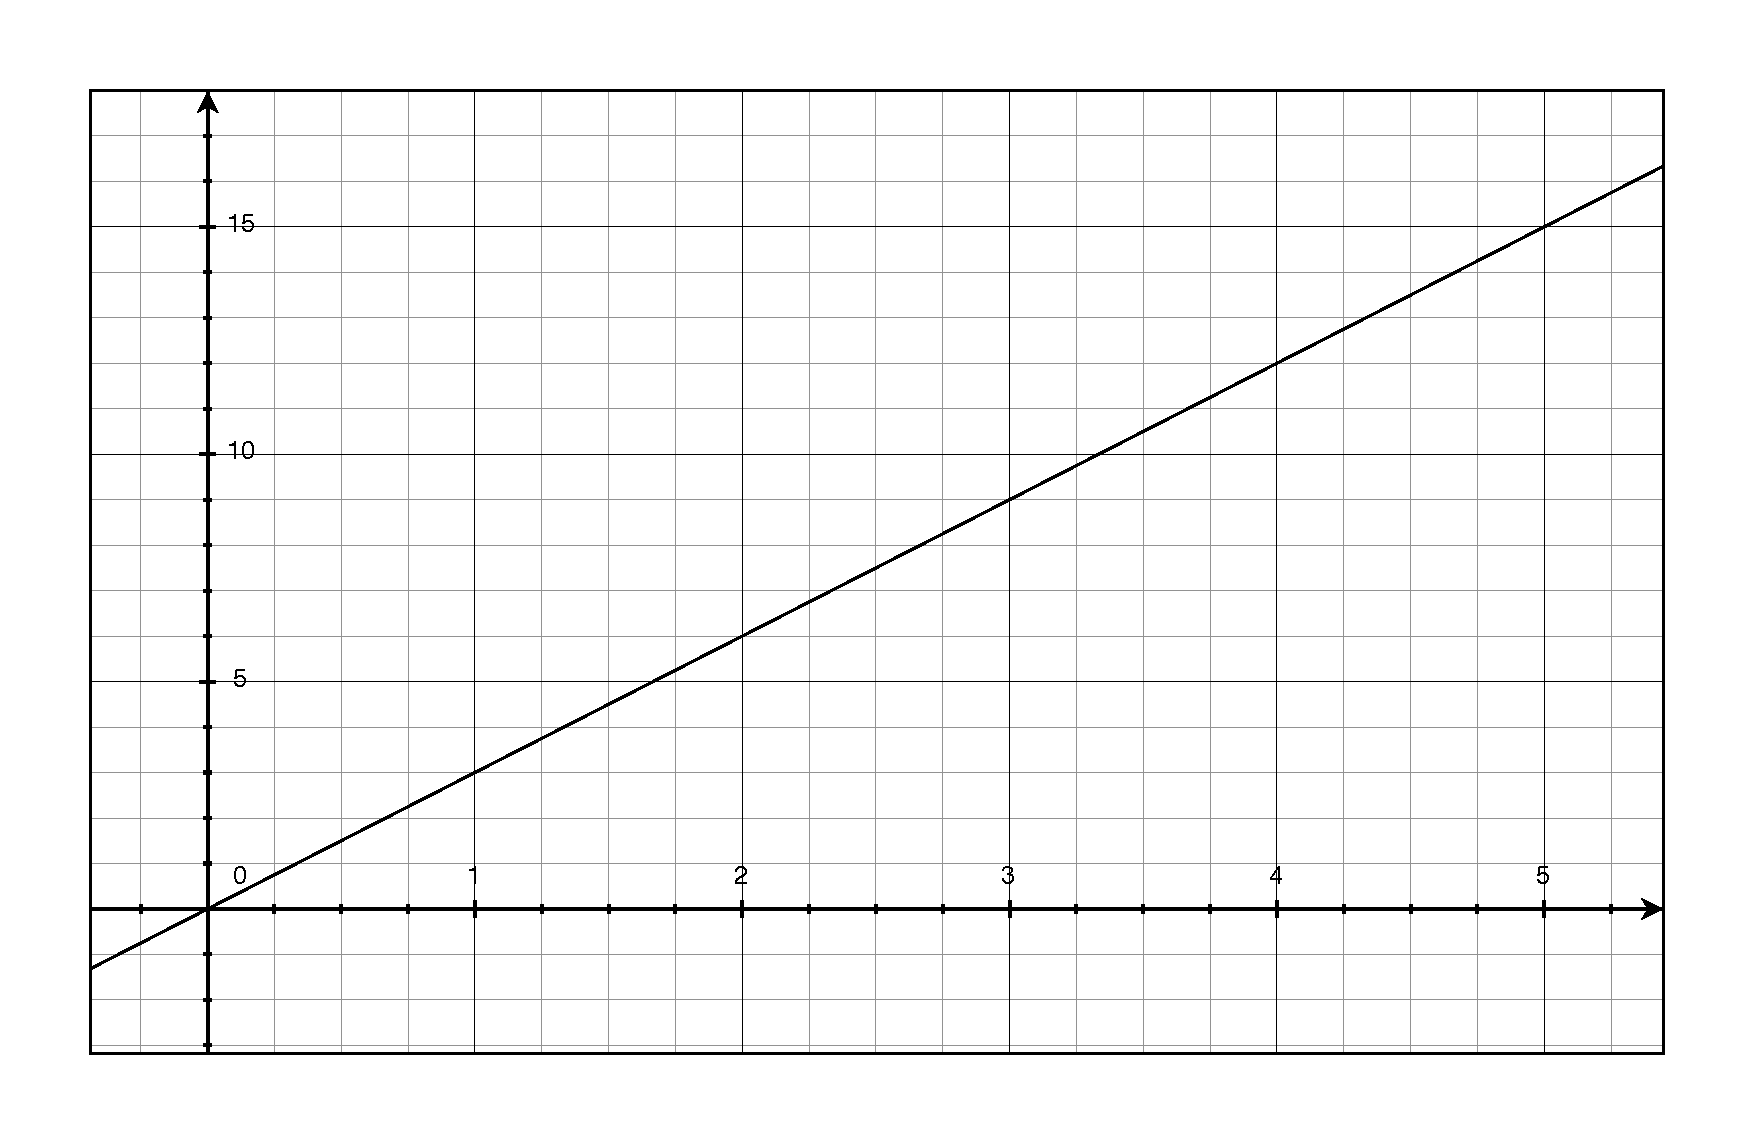
\includegraphics[scale=.3]{E18_a.eps}
  \caption*{E18 a}
\end{figure}

\begin{figure}[H]
  \centering
  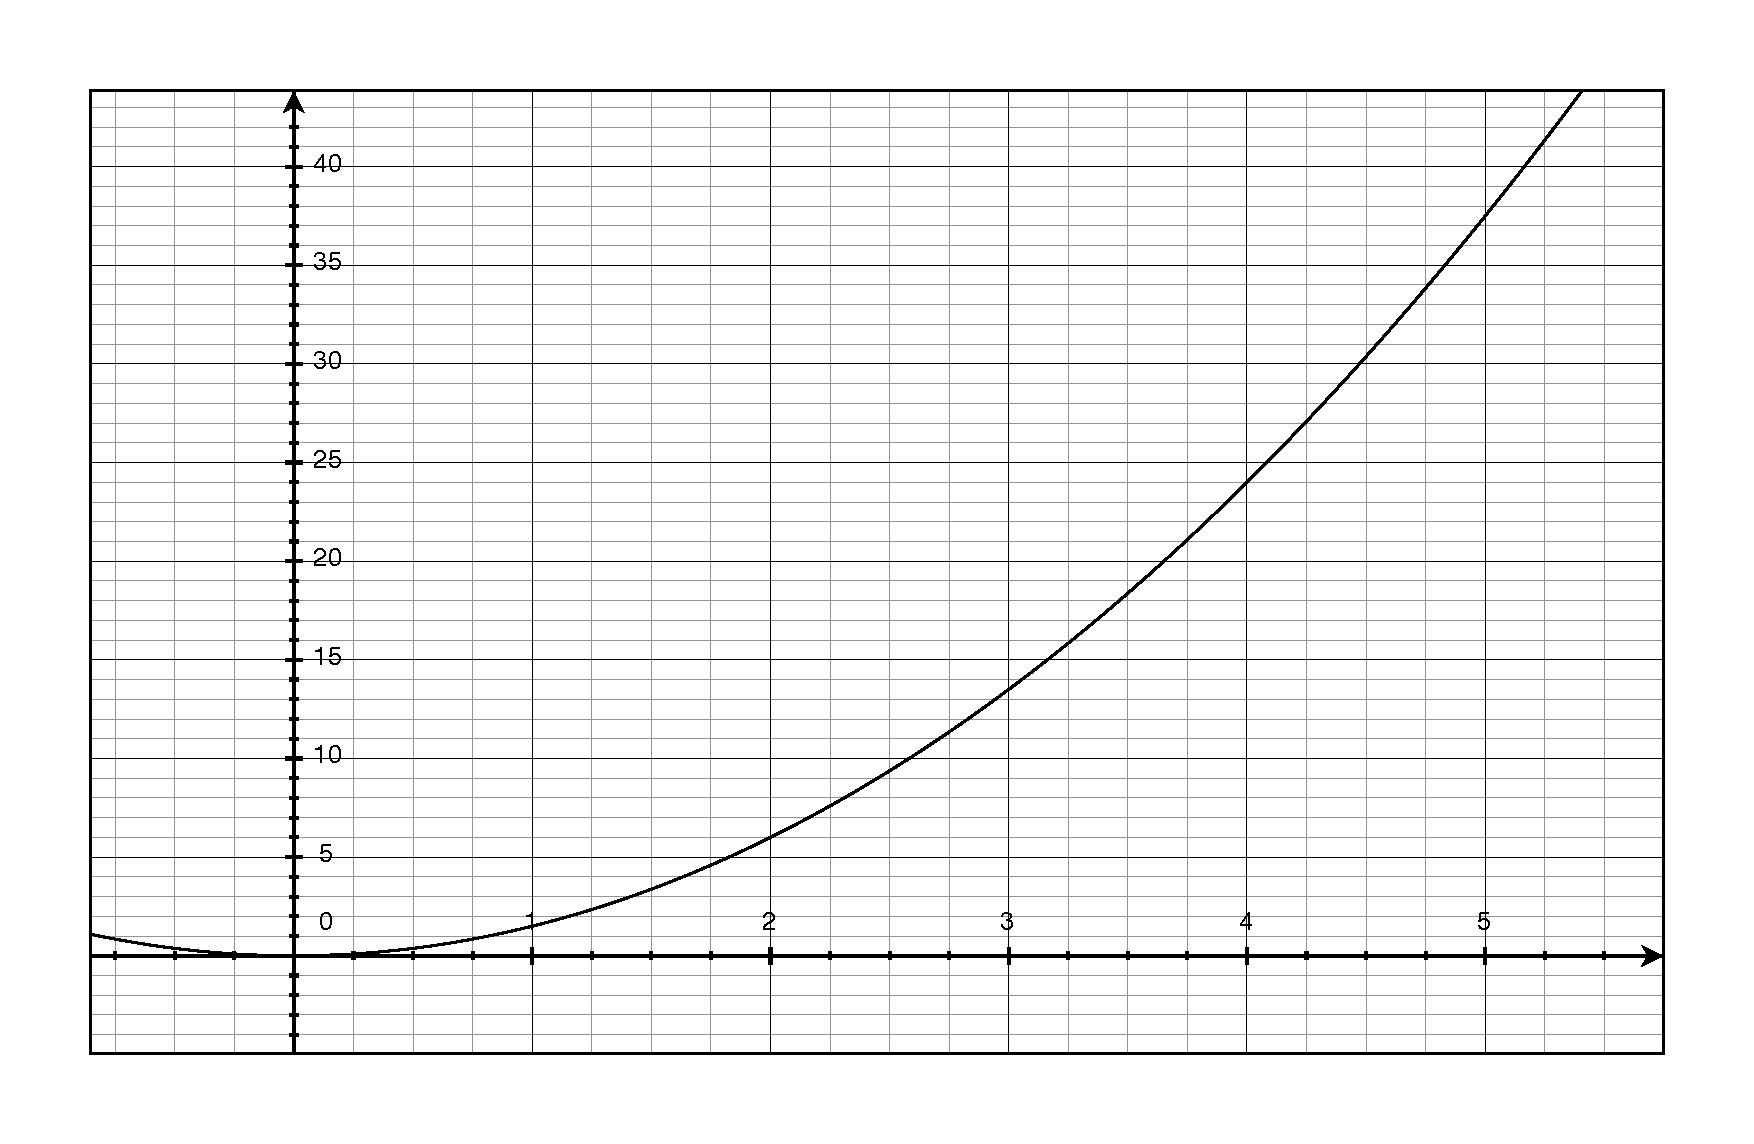
\includegraphics[scale=.3]{E18_b.eps}
  \caption*{E18 b}
\end{figure}


\item[SP2]
\begin{description*}
\item[a] 
\[
  \frac{4 \text{ m/s}}{4 \text{ s}} = 1 \text{ m/s}^2
\]

\item[b] 
\[
  \frac{8 \text{ m/s}}{4 \text{ s}} = 2 \text{ m/s}^2
\]

\item[c] 
\[
  \frac{12 \text{ m/s}}{8 \text{ s}} = 1.5 \text{ m/s}^2
\]

\item[d]
It is equal to the average.  The car spent 4 seconds at each acceleration.

\end{description*}

\end{description}

\subsection{Chapter 3}

\begin{description}
\item[Q9]
The acceleration is the slope of the velocity.  Since the slope of the velocity graph is changing, the acceleration is not constant.

\item[Q10]
\begin{description*}
  \item[a] yes.  Because of its initial velocity, it travels faster the entire time it is in the air and gets to the ground first.
  \item[b] no.  Both balls experience the same acceleration.
\end{description*}

\item[Q11]
At the start of its motion, the velocity is up and the acceleration is down.  The velocity decreases throughout the
flight, becoming zero and the peak and negative after the peak.  The acceleration is the same throughout.

\item[Q14]
no.  The acceleration is the same throughout the flight.

\item[Q20]
The direction of the velocity vector becomes more vertical as the ball travels through the air.  The x component of the
velocity vector remains the same (or decreases slightly, if you consider air resistance) while the y component of the
velocity vector increases.

\item[Q23]
The thing that affects the time of flight is the y-component of the velocity.  The ball that goes higher has a greater y
velocity and is in the air longer.

\item[E1]
\begin{description*}
\item[a]
\[
  v = (10 \text{ m/s}^2) (0.8 \text{ s}) = 8 \text{ m/s}
\]

\item[b]
\[
  v = (10 \text{ m/s}^2) (1.6 \text{ s}) = 16 \text{ m/s}
\]
\end{description*}

\item[E2]
\begin{description*}
\item[a]
\[
  v = \frac{1}{2} (10 \text{ m/s}^s) (0.8 \text{ s})^2 = 3.2 \text{ m}
\]

\item[b]
\[
  v = \frac{1}{2} (10 \text{ m/s}^2) (1.6 \text{ s})^2 = 12.8 \text{ m}
\]

\end{description*}

\item[E7]
\begin{description*}

\item[a] $v = (15 \text{ m/s}) - (10 \text{ m/s}^2) (1 \text{ s}) = 5 \text{ m/s}$

\item[b] $v = (15 \text{ m/s}) - (10 \text{ m/s}^2) (2 \text{ s}) = -5 \text{ m/s}$


\end{description*}

\item[E8]
\begin{description*}

\item[a] $y = (15 \text{ m/s}) (1 \text{ s}) - \dfrac{1}{2} (10 \text{ m/s}^2) (1 \text{ s})^2 = 10 \text{ m}$ (on the way up)
\item[b] $y = (15 \text{ m/s}) (1 \text{ s}) - \dfrac{1}{2} (10 \text{ m/s}^2) (2 \text{ s})^2 = 10 \text{ m}$ (on the way down)


\end{description*}

\item[E14]
\begin{description*}
\item[a] $v_y = (-10 \text{ m/s}^2) (0.6 \text{ s}) = -6 \text{ m/s}$
\item[b] The horizontal component hasn't changed and is still 5 m/s.
\end{description*}

\item[SP1]
\begin{description*}

\item[a] 
At the high point in its motion it is stopping and turning around so its velocity at this point is zero.

\item[b]
\begin{align*}
  v &= v_0 + at \\
  0 &= (16 \text{ m/s}) - (10 \text{ m/s}^2) t \\
  10t &= 16 \text{ s}\\
  t &= 1.6 \text{ s} \\
\end{align*}

\item[c]
\begin{align*}
  y &= v_0t + \frac{1}{2} at^2 \\
   &= (16 \text{ m/s}) (1.6 \text{ s}) - (5 \text{ m/s}^2) (1.6 \text{ s})^2 \\
   &= 12.8 \text{ m}
\end{align*}

\item[d]
\begin{align*}
  y &= v_0t + \frac{1}{2} at^2 \\
   &= (16 \text{ m/s}) (2 \text{ s}) - (5 \text{ m/s}^2)(2 \text{ s})^2 \\
   &= 12 \text{ m}
\end{align*}

\item[e]
The ball is moving down since it reached its peak at 1.6 s.

\end{description*}

\item[SP3]
\begin{description*}

\item[a] 
We are looking for the time when y is 0:

\begin{align*}
 y &= y_0 + \frac{1}{2} at^2 \\
 0 &= (0.8 \text{ m/s}) - (5 \text{ m/s}^2) t^2 \\
 5t^2 &= 0.8 \text{ s}^2 \\
  t^2 &= 0.16\text{ s}^2 \\
  t &= 0.4 \text{ s} \\
\end{align*}

\item[b]
Each ball is in the air for 0.4 s.

\begin{align*}
  x_1 &= (0.4 \text{ s}) (3 \text{ m/s}) = 1.2 \text{ m} \\
  x_2 &= (0.4 \text{ s}) (5 \text{ m/s}) = 2.0 \text{ m} \\
\end{align*}
\end{description*}

\end{description}

\fi

\section{Other Questions}

\begin{questions}

\question
Two divers run horizontally off the edge of a low cliff.  Diver 2 runs with twice the speed of diver 1.  When the 
divers hit the water, is the horizontal distance covered by diver 2:
\begin{description*}
  \item[a] the same as
  \item[b] twice as much as
  \item[c] four times as much as
\end{description*}
the distance covered by diver 1?

\begin{solution}
  Since the two divers are falling the same distance, they are in the air the same length of time.  Diver 1's horizontal
  velocity is twice diver 2's horizontal velocity, so he travels twice as far in this time.
\end{solution}

\question
Two divers dive off an overhang into a lake.  Diver 1 drops straight down and diver 2 runs off the cliff with an initial
horizontal speed of $v_0$.  Is the splashdown speed of diver 2:
\begin{description*}
  \item[a] greater than
  \item[b] less than
  \item[c] the same as
\end{description*}
the splashdown speed of diver 1?

\begin{solution}
When the divers land, they will have the same vertical velocity.  Diver 2, however, also has a horizontal component to
his velocity, so his total speed is greater.
\end{solution}

\question
A person flips a coin into the air and it lands on the ground a few feet away.  If the person were to perform an
identical coin flip on an elevator rising with constant speed, would the time of the flight be:
\begin{description*}
  \item[a] greater than
  \item[b] less than
  \item[c] the same as
\end{description*}
when the person was at rest?

\begin{solution}
There wouldn't be any change in the time of flight.  The speed of the elevator would add to the original speed the coin
was tossed, so the coin would move faster.  However, the coin has a shorter distance to travel because the elevator
moves upwards while the coin is in the air.  These two factors exactly cancel, and the coin toss would appear the same,
independent of the elevator's constant speed motion.

Galileo observed that the laws of physics work the same regardless of whether the observer is at rest (on the ground, in
this case) or moving at a constant speed (in the elevator, in this case).

\end{solution}

\question
An archer shoots an arrow horizontally at a target 15m away.  The arrow is aimed directly at the center of the target,
but it hits .5m lower.  What was the initial speed of the arrow?

\begin{solution}
The first thing to figure out is how long the arrow was in the air.  It had time to fall .5m, so:
\begin{align*}
  .5 &= \frac{1}{2} \cdot 9.8 t^2 \\
  t &\approx 0.32 \text{ s} \\
\end{align*}

In 0.32s, it traveled 15m, so the original speed was:
\[
  \frac{15}{0.32} \approx 47 \text{ m/s}
\]

\end{solution}

\question
An astronaut on the planet Zircon tosses a rock horizontally with a speed of 6.95 m/s.  The rock falls through a vertical
distance of 1.4 m, and lands a horizontal distance 8.75 m from the astronaut.  What is the acceleration of gravity on
Zircon?

\begin{solution}

First, we need to figure out how long the rock was in the air:
\[
  t = \frac{x}{v_x} = \frac{8.75 \text{ m}}{6.95 \text{ m/s}} \approx 1.26 \text{ s}
\]

Then we can use the constant acceleration formula to find $g$ for Zircon:
\begin{align*}
  y &= \frac{1}{2} \cdot g \cdot t^2 \\
  1.4 \text{ m} &= \frac{1}{2} \cdot g \cdot (1.26 \text{ s})^2 \\
  g &= 1.77 \text{ m/s}^2 \\
\end{align*}

\end{solution}

\question
In Syssex County, Delaware, a post-Halloween tradition is a contest in which contestants build devices to launch
pumpkins and compete for the greatest distance.  One winner shot his pumpkin 1246 m.  What is the minimum initial speed
needed for this shot?

\begin{solution}

Since velocity is a vector, the x and y components are given by:

\begin{align*}
  v_{0x} &= v_0 \cos \theta \\
  v_{0y} &= v_0 \sin \theta \\
\end{align*}

where $\mathbf{\vec{v}_0}$ is the initial velocity and $\theta$ is the launch angle.

The first thing to do is to figure out how long the pumpkin will be in the air.  There are two ways to do this.

One option is to figure out when the y coordinate is zero.  This happens at time 0, of course, before the launch.  It
also happens when the pumpkin hits the ground at the end of its flight.

\begin{align*}
  y = v_{0y} t + \frac{1}{2} at^2 \\
  0 = v_0 \sin \theta t + \frac{1}{2} at^2 \\
  0 = t \left( v_0 \sin \theta + \frac{1}{2} at \right) \\
\end{align*}

The solution at the end of the flight is given by:
\begin{align*}
  v_0 \sin \theta + \frac{1}{2} at &= 0 \\
  at &= -2 v_0 \sin \theta \\
  t &= - \frac{2 v_0 \sin \theta}{a} \\
\end{align*}

The other way to figure out how long the pumpkin is in the air is to figure out when $v_y$ is zero at the top of the
flight and multiply by 2.  Here's that approach:

\begin{align*}
  v_y &= v_{0y} + at \\
  0 &= v_0 \sin \theta + at \\
  t &= - \frac{v_0 \sin \theta}{a} \\
\end{align*}

Since this is the time to reach the top of the flight, you have to multiply by 2 to get the total flight time, so the
two approaches agree on the flight time.

Now we know the flight time, we need to figure out how far the pumpkin travels in the x direction in this time.  The
velocity in the x direction is constant and we can substitute in the expression for the total flight time.

\begin{align*}
  x &= v_{0x}t \\
   &= v_0 \cos \theta t \\
   &= v_0 \cos \theta \left( - \frac{2 v_0 \sin \theta}{a} \right) \\
   &= - \frac{2 v_0^2 \sin \theta \cos \theta}{a} \\
\end{align*}

As mentioned in the chapter, the greatest distance is reached with a launch angle of $45 \degree$.  So now we can plug
in all the numbers and solve for $v_0$:

\begin{align*}
   1246 \text{ m} &= - \frac{2 v_0^2 \sin 45 \degree \cos 45 \degree}{-9.8 \text{ m/s}^2} \\
   v_0 &\approx 110 \text{ m/s}
\end{align*}

\end{solution}

%% \question Find the $x$ and $y$ components of a vector $\vec{r}$ of magnitude $r = 75m$ if its angle relative to the x
%% axis is
%% \begin{parts}
%%   \part $30 \degree$
%%   \part $60 \degree$
%% \end{parts}

\end{questions}

\vspace{5.5 in}

\ifprintanswers
\else
\begin{em}
  Under a government which imprisons any unjustly, the true place for a just man is also a prison. The proper place
  to-day, the only place which Massachusetts has provided for her freer and less desponding spirits, is in her prisons,
  to be put out and locked out of the State by her own act, as they have already put themselves out by their
  principles. It is there that the fugitive slave, and the Mexican prisoner on parole, and the Indian come to plead the
  wrongs of his race, should find them; on that separate, but more free and honorable ground, where the State places
  those who are not with her, but against her---the only house in a slave State in which a free man can abide with honor.
\end{em}

\vspace{.2 cm}
\hspace{1.5 cm} --Henry David Thoreau, {\em Civil Disobedience}

\fi

\end{document}

